% ----------------------------------------------------
% Implementation
% ----------------------------------------------------

\chapter{PCB Construction, Adjustments and Code}\label{ch:implementation}

\section{PCB Design}

The probe, controller and gold electrodes were fabricated on \glspl{pcb}, which were designed using KiCad software and manufactured with JLCPCB.
The KiCad design files can be found in the Git repository linked in \refappx{appx:gitrepo}. 
The gold electrodes were trivial, only requiring a single layer \gls{pcb} with simple pads and traces.

The probe \gls{pcb} was the most complex.
It was fabricated on a 4-layer \gls{pcb} with dimensions of $50\times 50mm$, shown in \reffig{fig:probe-pcb}.
JLCPCB offered a discount for 4-layer \glspl{pcb} that were smaller than $50\times 50mm$ in size.
While the probe should ideally be as small as possible to fit through the ice core, it was not designed to be smaller than $50\times 50mm$ to allow for a more straightforward debugging process.

%chktex-file 44
\begin{figure}[ht]
    \begin{minipage}{0.5\textwidth}
        \centering
        \includegraphics[width=0.8\textwidth]{Figures/probe_pcb}
    \end{minipage}
    \begin{minipage}{0.5\textwidth}
        \centering
        \begin{tabular}{cl} \hline
            1 & Programmer Port \\ \hline
            2 & Test Points \\ \hline
            3 & Pressure Sensor in a Protective Housing \\ \hline
            4 & $11\times$ Gain Op-Amp \\ \hline
            5 & Titanium Electrode Port \\ \hline
            6 & Gold Electrodes \\ \hline
            7 & Unity Gain Buffer Op-amp \\ \hline
            8 & \gls{dac} and Buffer Transistor \\ \hline
            9 & \gls{uart} to \gls{rs485} Converter \\ \hline
            10 & \gls{rs485} Port \\ \hline
            11 & \gls{uart} Port \\ \hline
            12 & STM32F4 Microcontroller \\ \hline
            13 & \glspl{led} \\ \hline
        \end{tabular}
    \end{minipage}
    \caption{The probe PCB with the gold electrodes attached and some adjustments made}
    \label{fig:probe-pcb} %chktex 24
    \textit{Note 1: The rest of the titanium electrode ports are behind the gold electrode.} \\
    \textit{Note 2: The other \glspl{ic} present are the TS3A4751 switches.}
\end{figure}

The probe was designed with the resistance measuring circuitry, the temperature and pressure sensors, the microcontroller, the \gls{uart} to \gls{rs485} converter and the \gls{rs485} port mentioned in \refch{ch:design}.
The gold and titanium electrode ports, which were placed at the bottom of the probe, were designed to allow them to be soldered perpendicular to it.
The other methods of attachment all presented a fundamental disadvantage: connecting them with wires added extra resistance, and attaching them parallel to the board or perpendicular facing downwards was considered too complex.

Several adjustments were made to facilitate easier debugging
A \gls{uart} port was added next to the \gls{rs485} port to allow for data to be streamed to a computer using a \gls{uart} to \gls{usb} converter.
Both ports also had reverse polarity protection added to prevent unintentional board damage. 
\glspl{led} were added next to the microcontroller, and a programmer port and test points were added at the top of the board to allow for visual feedback and circuit analysis.
With the programmer and communication ports at the top of the board and the electrodes at the bottom, the probe could safely be submerged while transferring its data to a laptop.

The controller \gls{pcb} was fabricated on a 2-layer board, which is shown in \reffig{fig:controller-pcb}, as the components were too large to fit on a $50\times 50mm$ 4-layer board.
JLCPCB offered a similar discount for 2-layer \glspl{pcb} that were less than $100\times 100mm$ in area.
Ultimately, the controller dimensions were $100\times 60mm$, which could comfortably fit all the components while taking advantage of \texttt{JLCPCB}'s discount.

\begin{figure}[ht]
    \begin{minipage}{0.5\textwidth}
        \centering
        \includegraphics[width=\textwidth]{Figures/controller_pcb_final}
    \end{minipage}
        \begin{minipage}{0.5\textwidth}
            \centering
            \begin{tabular}{cl} \hline
            1 & Salinity 7-Segment Display \\ \hline
            2 & Depth 7-Segment Display \\ \hline
            3 & Rotary Switches \\ \hline
            4 & Power Input \\ \hline
            5 & \gls{uart} to \gls{rs485} Converter \\ \hline
            6 & \gls{rs485} Port \\ \hline
            7 & \gls{uart} Port \\ \hline
            8 & Input Buttons \\ \hline
            9 & Programmer Port \\ \hline
            10 & SD Card Port \\ \hline
            11 & STM32F0 Microcontroller \\ \hline
            12 & \glspl{led} \\ \hline
        \end{tabular}
    \end{minipage}
    \caption{The controller PCB with the rotary switch caps attached}
    \label{fig:controller-pcb} %chktex 24
\end{figure}

The controller was designed with the buttons, the rotary switches, the 7-segment displays, the \gls{uart} to \gls{rs485} converter, and the \gls{rs485} port mentioned in \refch{ch:design}.
The 7-segment displays were designated to display the salinity and depth of the water by default using silkscreen text, but they could be changed to display anything using software.
The components were placed user-friendly, allowing for easy use of the buttons and rotary switches.
Similarly to the probe, \glspl{led}, a \gls{uart} port and a programmer port were added to the board to allow for debugging of the board.
It should be noted that an SD Card Port was added for future development and testing but was not utilised during this project.

\section{PCB Adjustments}

Three adjustments were made to the probe \gls{pcb} to ensure it functioned as required, excluding the soldering of headers and the gold electrodes.
Firstly, one of the microcontroller's pins was unconnected to power and was corrected by soldering a wire between it and a pin with power, which can be seen on the left of the microcontroller.
Secondly, the footprint of the pressure sensor was horizontally reversed, which was corrected by flipping and soldering the depth sensor vertically.
A protective case was added around the pressure sensor to prevent it from being damaged during testing.
The casing would later function as the support for the waterproof membrane mentioned in \refsec{sec:temp-depth-measurement}.

Lastly, both op-amps were incorrectly chosen as they required a rail-to-rail voltage of $6V$ to operate, higher than the $3,3V$ provided.
Thus, they were replaced with an alternative op-amp model with the same footprint.
The temperature sensor also had an incorrect footprint, but this could not be rectified as it was discovered after the board was fabricated. 
Thus, the temperature sensor was not soldered to the board.
The pressure sensor's onboard temperature sensor was used instead.

The controller \gls{pcb} required no soldering adjustments.
There was a minor error in the pin assignments of the rotary switches, but this was corrected in the software and did not require any hardware changes.
Switch caps were 3D printed and attached to rotary switch shafts to make them easier to turn, making the controller more user-friendly.

\section{Probe Code}

The significant steps in measuring salinity are measuring the water's conductivity, temperature and pressure and then calculating its salinity.
An overview of this process is shown in \reffig{fig:probe-code-flowchart}.

\begin{figure}[ht]
    \centering
    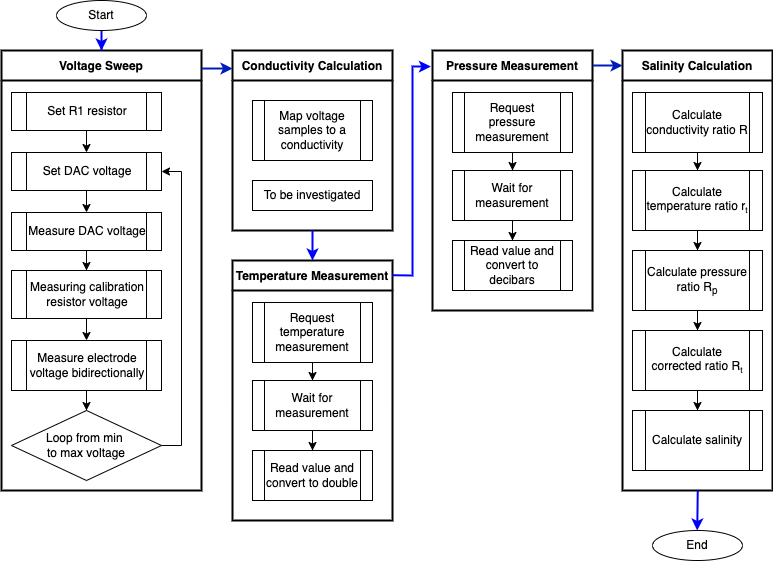
\includegraphics[width=1\textwidth]{Figures/probe_flowchart}
    \caption{The flowchart for the probe code that measures salinity.}
    \label{fig:probe-code-flowchart} %chktex 24
\end{figure}

The conductivity measurement was aimed at repeating the methodology that \refref{benjankar_ec_based_salt_measurement_2021} employed.
This requires a voltage sweep of the water sample, which is then mapped to a conductivity.
This devices specific mapping will have to be determined experimentally, as it is unique for different electrode sizes and materials.
The voltage sweep is achieved by incrementing the output of the \gls{dac} from a given start to end voltage.
At each step, the output of the \gls{dac} and the voltage drop across the calibration resistor and the electrodes are recorded.

To determine the resistance measuring accuracy, the resistance across the electrodes $R_E$ was calculated using the voltage drop across the electrodes and across the calibration resistor $R_C$, as shown in \refeqn{eqn:electrode-calib-resistance} to \refeqn{eqn:electrode-calib-resistance-final}.
The electrode resistances $R_E$ was calculated for each voltage sample and then averaged.

\begin{align}
 V_{ratio} &= \lfrac{V_{DAC}A_{11}A_{ADC}\lfrac{R_E}{R_1 + R_E}}{V_{DAC}A_{11}A_{ADC}\lfrac{R_C}{R_1 + R_C}} = \lfrac{\lfrac{R_E}{R_1 + R_E}}{\lfrac{R_C}{R_1 + R_C}} \label{eqn:electrode-calib-resistance} \\
 \lfrac{R_E}{R_1 + R_E} &= V_{ratio} \lfrac{R_C}{R_1 + R_C} \rightarrow k \label{eqn:electrode-calib-resistance-simplified} \\
 R_E &= \lfrac{kR_1}{1 - k} \label{eqn:electrode-calib-resistance-final}
\end{align}

This method of calculating resistance using a voltage ratio with a known resistance allows the probe to nullify all scalar inaccuracies in the circuit, including the \gls{dac}, \gls{adc} and op-amp gain error, as they will be present in both voltage measurements.
However, this method is still vulnerable to offset inaccuracies, including \gls{dac} and \gls{adc} offset errors, op-amp input offset and input bias currents, the $R_1$ resistance errors and the resistance added by the switches and traces.

As previously mentioned, the pressure and temperature measurements are taken from the WF183DE pressure sensor.
This sensor operates similarly for both measurements: a request is made to make a measure, it can then be polled until the measurement is ready, and then the measurement can be read.

Once the conductivity, temperature and pressure measurements are taken and converted into the required units of $Sm^{-1}$, $\degree C$ and $dbar$ respectively, salinity can be calculated as shown in \refsec{sec:salinity-conductivity-relationship}.
Additionally, if requested, any of the temperature, depth, resistance, or conductivity measurements can be calculated individually and transmitted to the controller.

\section{Controller Code}

The controller's primary function for the prospective user was to instruct the probe to take a measurement and display it. However, the controller was given additional functionality for testing and investigation purposes, which allowed the controller to update the probe's configuration.

The common-cathode 7-segment displays displayed the various measurements from the probe.
The displays' digits were individually written to by writing the digit code and keeping the corresponding digit's cathode low while keeping the others high.
A timer controlled \gls{dma} was used to write to each digit in quick succession, giving the illusion of all the digits being on simultaneously.

The leftmost rotary switch was used to navigate the menu, which consisted of the default showing both salinity and depth, individual measurements of temperature, depth, resistance, conductivity, and salinity, and the probe's configurable parameters.
The menu names were displayed on the top 7-segment display, and the selected menu item was displayed on the other.
This created some limitations on what could be displayed. 
For instance, the best display of the word `temperature' was `teP', but all menu items had a unique, relatively clear name.

When the user selected a measurement menu item, the top switch was configured to request that measurement from the probe and display it; when the user selected a configuration menu item, the top switch was configured to update the probe's configuration.
The other two rotary switches adjusted the probe's configurable parameters, further discussed in \refsec{sec:board-to-board-communication}.
The bottom switch was configured to reset the probe and the controller should an error occur.

\section{Board-to-Board Communication}\label{sec:board-to-board-communication}

The probe and controller communicate using half-duplex \gls{rs485}, which is converted on both sides to \gls{uart}.
This makes the protocol effectively half-duplex \gls{uart} communication from the perspective of the microcontrollers.
The probe was configured to be in receive mode, where it would perpetually wait for a one-byte command from the controller.
All the possible commands and expected transactions are shown in \reffig{fig:rs485-flowchart}.

\begin{figure}[ht]
    \centering
    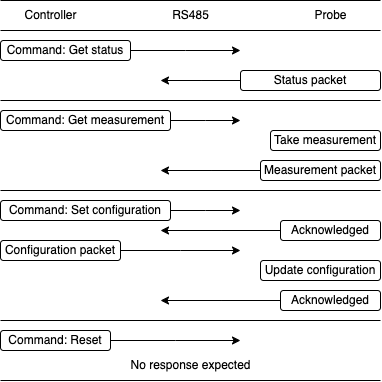
\includegraphics[width=0.5\textwidth]{Figures/rs485_flowchart}
    \caption{The flowchart for the board-to-board communication protocol denoting the four transaction types. The arrows denote the direction of the packets being sent over the \gls{rs485} link.}
    \label{fig:rs485-flowchart} %chktex 24
\end{figure}

While not directly available to the user, the controller could request a status byte to which the probe would respond with \textit{idle}, \textit{busy} or \textit{error} depending on its state.
This allowed for some simple error checking and communication flow, which could be integrated into more robust error handling in the future.
When the user requests a measurement, the controller sends the corresponding request command, to which the probe will respond with the measurement data.
The data was returned as a 3-byte, fixed-point float.

When the user requested a configuration update, the controller transferred a configuration packet using the expected transaction.
Once the probe was entirely cast in epoxy resin, the configuration could only be updated this way, so all possibly useful, configurable parameters are included.
This included which electrode to use (including whether to use the fringe shield), the $R_1$ resistor to use, the directionality of the resistance measurement (unidirectional or bidirectional), the voltage sweep start, end and number of steps, among other parameters.
Some parameters, such as the directionality, were unlikely to be changed from their default value (bidirectional) but were included to cover any unforeseen circumstances.

When the user resets the boards using the controller's bottom switch, a reset command was sent to the probe before the controller reset itself.
This command allows for resetting the probe should a system error occur.
However, this only works provided the \gls{rs485} link is still operational.
Otherwise, the entire system must be powered off and on again to reset the probe.
The reset on both microcontrollers is triggered using software to set the \gls{sys_reset_req} bit in the \gls{scb} register, which triggers a system reset similar to pulling the reset pin low.

\section{Probe Epoxy Casting}\label{sec:probe-epoxy-casting}

The circuitry on the probe had to be protected from the salt water while the electrodes were submerged, which was achieved using \textit{Kristal 20} epoxy resin.
Before casting the epoxy, the \gls{rs485} ports on the controller and probe were connected using a multicore cable, which connected their power, ground and the \gls{rs485} data lines, which can be seen in \reffig{fig:epoxy-top}.
A casting mould was created using acrylic sheets, which are commonly used for epoxy moulds as they tend not to stick to the epoxy.
The sheets were cut and secured using hot glue, as seen in \reffig{fig:epoxy-side}.

\begin{figure}[ht]
    \begin{minipage}{0.49\textwidth}
        \centering
        \includegraphics[width=0.84\textwidth]{Figures/epoxy_casting_top}
        \caption{A top view of the probe casting mould, the controller and the connecting cable.}
        \label{fig:epoxy-top} %chktex 24
    \end{minipage}
    \begin{minipage}{0.49\textwidth}
        \centering
        \includegraphics[width=\textwidth]{Figures/epoxy_casting_side}
        \caption{A side view of the probe casting mould showing the gold electrode spacers.}
        \label{fig:epoxy-side} %chktex 24
    \end{minipage}
\end{figure}

The gold electrodes were precisely spaced using 3D-printed spacers, which were attached during the casting process and removed once the epoxy had cured.
Lastly, two areas of the probe still needed to be accessed: the programmer and \gls{uart} ports and the titanium electrode ports.
This would simplify further testing and allow the titanium electrodes to be optimally spaced through experimentation instead of estimations.
These areas were isolated using \textit{Prestick}, a rubber-based reusable putty adhesive. 
The adhesive was removed after the epoxy had cured, allowing access to the aforementioned areas.

The probe was removed from the mould after the epoxy had cured, shown in \reffig{fig:probe-final}.
The \textit{Prestick} adhesive was relatively easy to remove, and the desired areas were still accessible, allowing the titanium electrode to be added.
Titanium is challenging to solder, requiring a complex process and advanced machinery that was not available for this project~\cite{totalmateria_joining_titanium_2005}.
Instead, thin copper wire was tightly wrapped around the last $5mm$ of the titanium electrode, which was folded over to secure the copper wire, as shown in \reffig{fig:titanium-electrodes}.
This configuration made connecting the electrodes to their ports easy using standard soldering and provided a continuous connection between the probe and the titanium electrode.

\begin{figure}[ht]
    \begin{minipage}{0.5\textwidth}
        \centering
        \includegraphics[width=0.65\textwidth]{Figures/probe_final}
        \caption{The probe after the epoxy casting process with the titanium electrodes and pressure sensor's flexible membrane attached.}
        \label{fig:probe-final} %chktex 24
    \end{minipage}
    \begin{minipage}{0.5\textwidth}
        \centering
        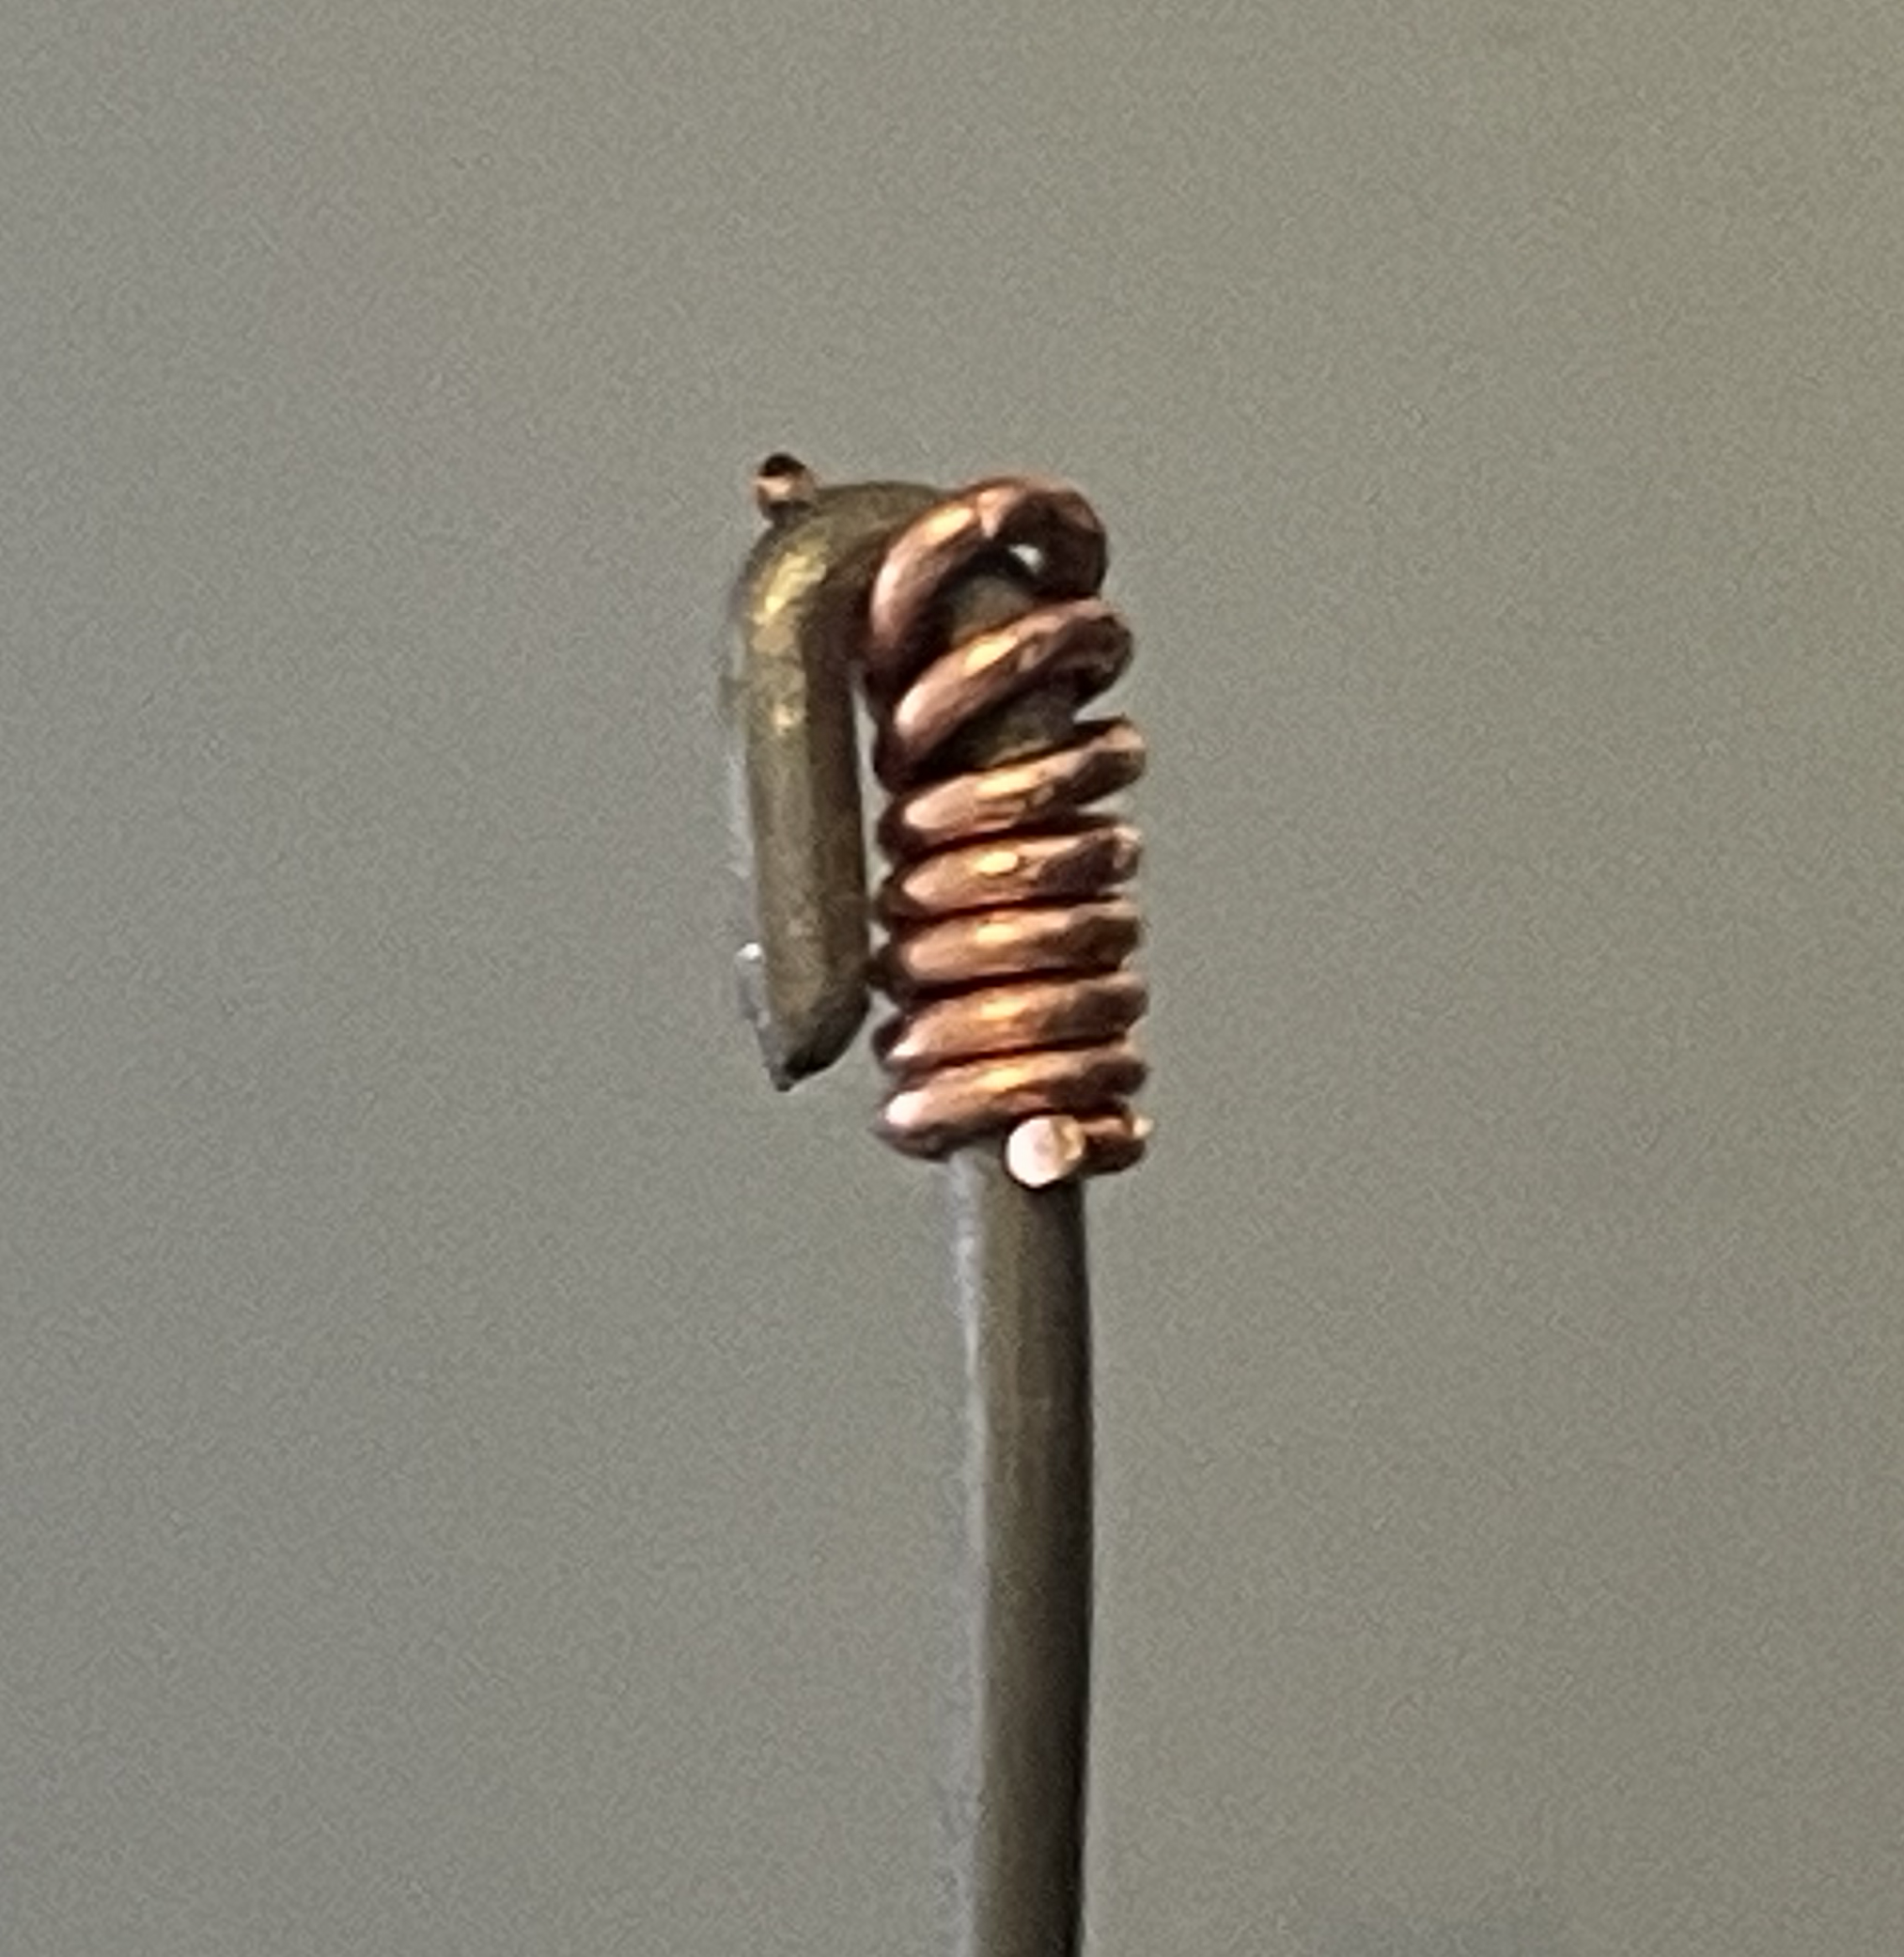
\includegraphics[width=0.75\textwidth]{Figures/titanium_electrode}
        \caption{A close-up of the titanium electrode with the copper wire attached.}
        \label{fig:titanium-electrodes} %chktex 24
    \end{minipage}
\end{figure}

The unevenness of the mould and the hot glue created some rough edges along the epoxy.
These could be laser cut to a smooth finish for the final product, but this was considered unnecessary for the experiments conducted in this project.

Lastly, hot glue was used to attach a flexible membrane to the pressure sensor's protective casing.
The membrane was taken from the packaging of the gold electrode \glspl{pcb} as it was readily accessible and had the required flexibility and durability to prove the concept.
The final device would require further investigation into a more suitable material.
The protective casing was also coated in a thin layer of hot glue as the 3D printing process used to create it had a small probability of being porous.